Avtomatska stružnica je stružnica, kjer so vsi
gibi, kot na primer vključevanje glavnega vretena
in podajalnih gibanj, sprememba števila vrtljajev
glavnega vretena in podajalnih hitrosti, vpenjanje
obdelovanca, vključevanje dodatnih naprav in drugo,
v celoti avtomatizirani. Lahko se krmilijo s krivuljno gredjo,
servo ali koračnimi motorji, hidravlično ... Ob spremembi oblike
obdelovanca je potrebno dolgotrajno nastavljanje krmiljenja.
Ko je to urejeno, delavec samo nadzoruje delovanje
in občasno izmeri kose ter vloži novo palico materiala
v podajalec.

Na avtomatskih stružnicah največkrat obdelujemo paličast
material, ki ga dovajamo v stroj skozi posebno vodilno
cev, ki je v sredini glavnega vretena. Lahko obdelujemo tudi
polizdelke v obliki odkovkov, ulitkov, sintranih ali ostalih polizdelkov.
Za te je potrebno dodati naprave za vstavljanje posamičnih kosov,
ki so lahko tudi robotske roke.
Če so polizdelki večji ali
nerodnih oblik, je njihovo vstavljanje lahko zelo težavno
in jih zato vpnemo ročno. Seveda pa v takem primeru
ne moremo več govoriti o avtomatu, temveč o
polavtomatskem stroju.

\noindent Avtomatske stružnice delimo na:
\begin{itemize}
	\item Enovretenske
	\item Večvretenske
\end{itemize}

Spodaj sta obe vrsti avtomatskih stružnic. Levo, na Sliki \ref{eno_vretenska_struznica}
je prikazana enovretenska stružnica, desno, na Sliki \ref{vec_vretenska_struznica}
pa je prikazana večvretenska stružnica.

\begin{multicols}{2}
	\begin{figure}[H]
		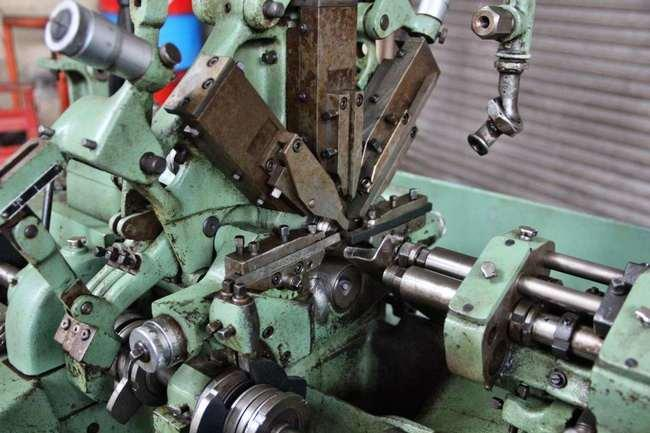
\includegraphics[width=\linewidth]{eno_vretenski_avtomat.jpg}
		\caption{Enovretenska stružnica
			\cite{eno_vretenska_struznica}}
		\label{eno_vretenska_struznica}
	\end{figure}

	\columnbreak

	\begin{figure}[H]
		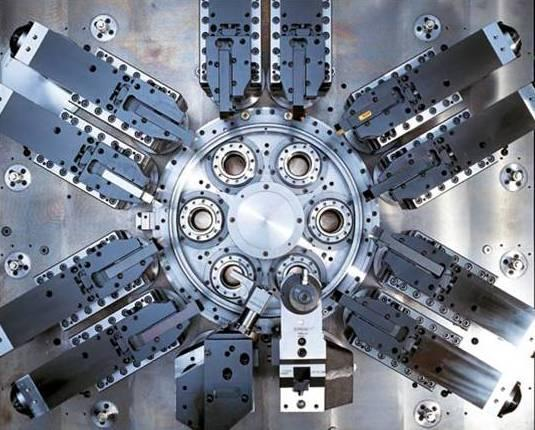
\includegraphics[width=\linewidth]{vec_vretenska_struznica.jpg}
		\caption{Večvretenska stružnica
			\cite{vec_vretenska_struznica}}
		\label{vec_vretenska_struznica}
	\end{figure}
\end{multicols}
